\chapter{State of the art}
\label{Chap2}
\section{Selective laser melting technology}
Selective laser melting (SLM) - also referred to as direct metal laser sintering (DMLS) - is an additive manufacturing  (AM) technique making use of a high power-density laser that locally melts powder materials.%Layers are progressively piled up, in order to create a 3D part. 
 When a layer of powder has been melted, a new layer is spread on top of the previous one, and is in turn melted, in order to progressively build a 3D object. The technique is illustrated on figure \ref{fig:SLM} \parencite{LEITZ2017331}. The materials used include mostly metals but also ceramics and composites. Parts to build must first be drawn in a computer-aided design (CAD) software and broken down in 2D slices, each one corresponding to a powder layer. During the process, the oxygen pressure $p_{O_2}$ must be kept low to prevent the oxidation of the metal. A shielding gas - such as argon - is thus used to fill the build chamber at all time, while $p_{O2}$ is monitored.   \\

\begin{figure}[ht]
\centering
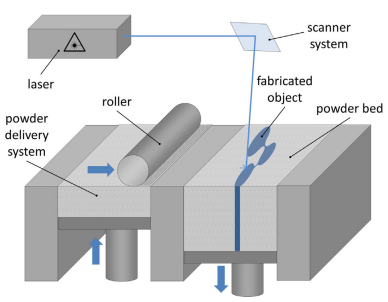
\includegraphics[scale=0.7]{Images/SLM}
\decoRule
\caption[Selective laser melting technology principle]{Selective laser melting technology principle (from Leitz et al., 2017 \parencite{LEITZ2017331}).}
\label{fig:SLM}
\end{figure}

SLM is still a young technology. Its popularity only increased significantly over the last decade, as depicted by figure \ref{fig:Evol}. Works concerning AlSi10Mg began to emerge noticeably in 2014. The technique usage spread rapidly in many sectors: biomedical, heat exchangers, aerospace and automotive - to name just a few \parencite{Yap}. This is due to the numerous appeals of SLM compared to the other technologies, including:\\

\begin{itemize}
\item Geometrical flexibility: parts can be designed with thin walls or even with hidden cavities and/or channels. This offers promising prospects regarding light-weight potentials for parts solicited mechanically \parencite{Lippert};
\item Increased reliability of the parts \parencite{Haase};
\item Reduced equipment costs \parencite{Hoeges};
\item Better operational efficiency: the fabrication is quick and easy which reduces time-to-market as well as assembly times and capital tied up in stocks \parencite{Hoeges};
\item Individual production facilitation \parencite{Haase};
\item Reduced material waste and better energy usage: the process is  environmentally friendly as a whole \parencite{Haase}.
\end{itemize}

\begin{figure}[ht]
\centering
\noindent\makebox[\textwidth]{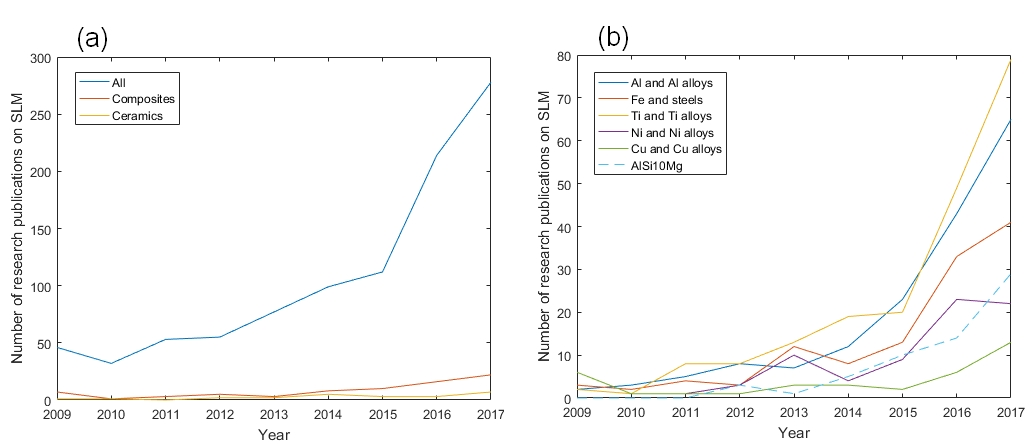
\includegraphics[scale=0.55]{Images/Evol}}
\decoRule

\caption[(a)Research publications on SLM of ceramics, composites and all materials types combined. (b)Research publications on SLM of different metallic materials]{(a)Research publications on SLM of ceramics, composites and all materials types combined. (b)Research publications on SLM of different metallic materials. Data are derived from the research publications on SLM, LaserCusing and DMLS existing on ScienceDirect website.}
\label{fig:Evol}
\end{figure}

The properties of parts produced through SLM stem from the coupled effects of a great deal of parameters (see figure \ref{fig:param} ) \parencite{Aboulkair140820}.  %Les caractérisitiques des pièces produites grâce à la fusion laser sélective (SLM) sont le fruit de l'action simultanée et couplée d'un grand nombres de paramètres (see figure \ref{fig:param} ) \parencite{Aboulkair140820}.
Results are very sensitive to their variations. The process parameters must thus be monitored thoroughly. This complicates the search for their optimisation, still not fully resolved for aluminium alloys.\\%.Les résultats sont très sensibles à leurs variations et il est donc nécessaire de les contrôler méticuleusement. Pour ces raisons, il n'est pas simple d'étudier leurs impacts.\\
\begin{figure}[ht]
\centering
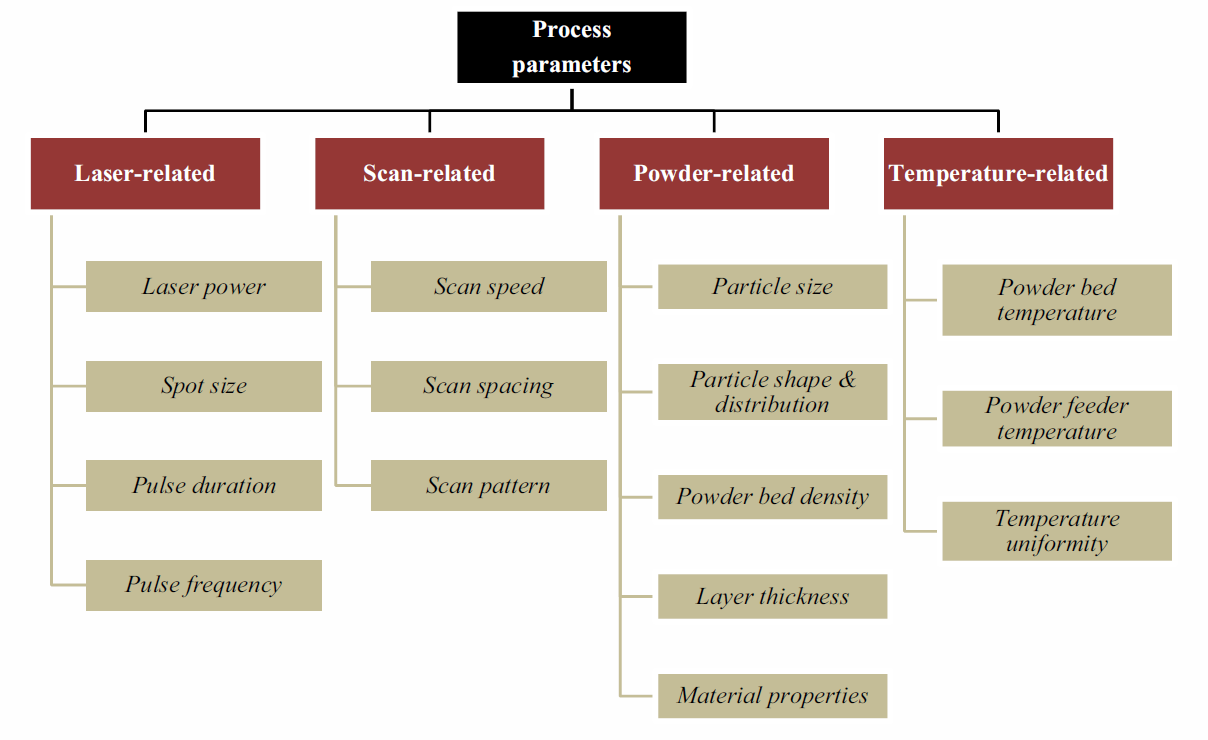
\includegraphics[scale=0.37]{Images/Param}
\decoRule

\caption[Parameters involved in SLM]{Parameters involved in SLM (from Aboulkhair et al., 2014 \parencite{Aboulkair140820}).}
\label{fig:param}
\end{figure}

In recent years, works aiming at facing this challenge multiplied. The minimisation of the porosity is at the center of attention. It is indeed closely related to the quality of the mechanical properties. As porosity contributes to lowering the load-bearing surface, it reduces the apparent material strength. It was also observed to have a critical influence on the fatigue life of the produced parts. Their lifetime is especially diminished if the values of pores amount and size go beyond a certain threshold \parencite{Brandl121509}. Studies investigating the effects of various parameters on the AlSi10Mg fabrication through SLM abound in the literature.\\

\section{AlSi10Mg alloy}
%\textcolor{red}{Parler de l'AlSi10Mg; quel est l'interet de travailler avec? Difficultés? (reflectivité etc).. Qu'est ce qui existe en coulé, forgé etc}\\
%\textcolor{red}{Microstructure homogène, diagramme de phase}\\

AlSi10Mg is a popular casting alloy. It is well known for its high strength-to-density ratio, thermal properties and post-processing flexibility. This makes AlSi10Mg a material of choice in automotive, aerospace, automation, chemical and food industries \parencite{Kempen110817}. Specific applications contain housings, ductwork, engine parts, production tools and molds, both for prototyping and manufacturing purposes. \parencite{Alu}. Processing the alloy with SLM is quiet easy due to the small difference between its solidus and liquidus temperatures \parencite{Kempen110817}. Nevertheless, high laser power is needed to compensate the energy losses due to the high reflexivity (91\%) and the fast heat dissipation resulting from the consequent thermal conductivity (146 [$\frac{W}{mK}$]) \parencite{aboulkhair2016}.\\

%\textcolor{gray}{Kempen dans "PROCESS OPTIMIZATION AND MICROSTRUCTURAL ANALYSIS FOR SELECTIVE LASER
%MELTING OF AlSi10Mg ":}
%
%\textcolor{gray}{Aluminium as a lightweight material is very attractive for the production of parts that require good
%mechanical properties in combination with a low weight. The main focus lies on Al-Si alloys, since they are
%casting alloys that are also suitable for welding. AlSi10Mg, which can be hardened by applying a specific heat
%treatment, is relatively easy to process by laser applications due to the small difference between liquidus and
%solidus temperature compared to high strength aluminium-alloys [2]. The AlSi10Mg alloy is frequently used in
%aerospace, automotive, chemical and food industry. Its composition according to ISO 3522 can be found in
%Table 1 [4]. Alloying the magnesium to the Al-Si alloy enables precipitation of Mg2Si which will strengthen the
%matrix without compromising the other mechanical properties to a significant extent.}\\

The most determinating property of the alloy is its composition. As it can be observed on the phase diagram of figure \ref{fig:phase_diagram}, and by assuming that the small concentrations of magnesium and impurities do not displace too much the diagram, AlSi10Mg has an hypo-eutectic concentration. Thus, the first solid to form during cooling is made of $Al-\alpha$ phase, followed by the formation of an eutectic compound. The addition of magnesium also permits the precipitation of Mg2Si which increases the strength of the material, without affecting significantly the other mechanical properties \parencite{Kempen110817}.\\

\begin{figure}[ht]
	\centering
	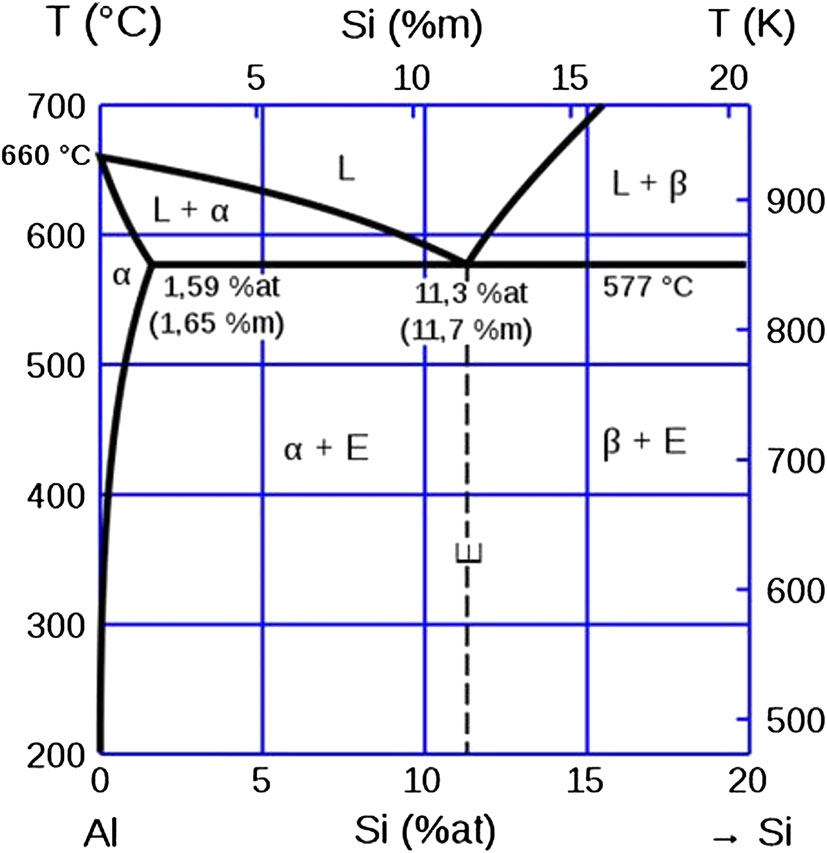
\includegraphics[scale=0.35]{Images/phase_diagram}
	\decoRule
	\caption[Phase diagram of Al-Si alloy near the eutectic]{Phase diagram of Al-Si alloy near the eutectic (from Rosenthal et al., 2014 \parencite{Rosenthal14}).}
	\label{fig:phase_diagram}
\end{figure}

Nevertheless, knowing the composition is not sufficient to predict the microstructure of the fabricated alloy. It depends heavily on the manufacturing process.  As shown in figure \ref{fig:micro_cast}, casting results in the formation of lamellar precipitates of Si-phase, measuring several tens of micrometers and floating in an Al matrix. In the first image of figure \ref{fig:micro_am}, we can observe a completely different macrostructure for a SLM manufactured sample at the same scale as the cast alloy. It consists of a stacking of successive scan tracks, that solidified following the laser passage, layer after layer. Its exact shape is dictated by the various parameters of the SLM process, which will be discussed in the Section \ref{pp}.\\

By zooming in, we see that those scan tracks are characterised by a very fine microstructure: cells of Al, measuring 1$\mu m$ or less, separated by a spider web-like network of Si. Those two were the only phase that were detected with XRD by Thijs et al. (2013) \cite{Thijs13}. This fineness is due to the intense thermal gradients appearing in the melt pool left behind the laser: they allow a particularly fast cooling (up to $10^5$ K/s \cite{PRASHANTH14}) and solidification, which do not let time for alloying elements to diffuse over much distance. However, this microstructure is not homogeneous across the whole part: the section of a scan track can be separated in 3 roughly concentric zones.\\

\begin{figure}[ht]
	\centering
	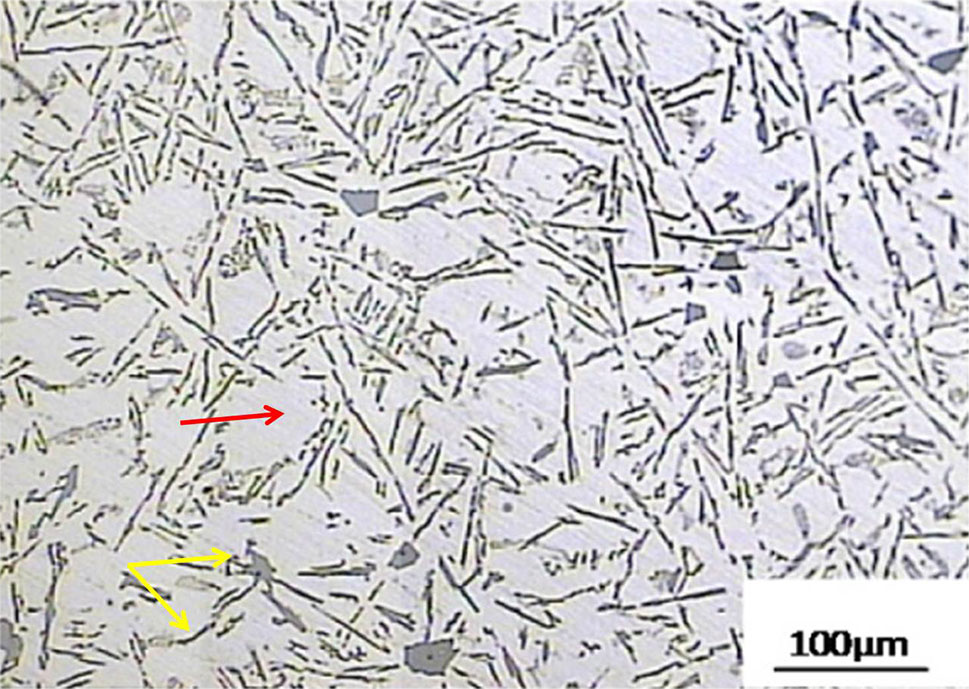
\includegraphics[scale=0.30]{Images/micro_cast}
	\decoRule
	\caption[Common microstructure of an Al-Si cast alloy]{Common microstructure of an Al-Si cast alloy, with the red arrow pointing to the Al matrix, and the yellow one to the Si lamellae (from Wang et al., 2012 \parencite{Wang12}).}
	\label{fig:micro_cast}
\end{figure}

First, there is the fine zone which is the result of the melt pool core solidification. The cellular dendrites start to grow from the melt pool edge resulting in elongated  cells, and converge towards the centre where they are more isotropic. Around it, near the boundary, lies the coarse zone with larger cells and thicker lamellae. According to Uzan et al. (2017) \cite{UZAN2017229}, the difference of microstructure is simply due to lower solidification rates ; the hot zones in the previous layer reduce the temperature gradient. Just outside the melt pool, in previously solidified tracks, lies a heat-affected zone(HAZ). Although it remains at least partially solid during the previous laser passage, temperature rises enough to allow Si to diffuse and coarsen into globular particles, breaking the cellular structure. It is from this specific microstructure that arise all the mechanical properties of the fabricated part, which will be presented in Section \ref{MMABMP}.\\

The impact of heat treatments on the microstructure is well known. The higher the temperature at which the material is exposed, the more pronounced the silicon spheroidization (see figure \ref{fig:microTT}) \parencite{aboulkhair2017}. This microstructure change heavily impacts the material mechanical properties, as discussed in section \ref{SOTAPT}.\\


\begin{figure}[ht]
	\centering
	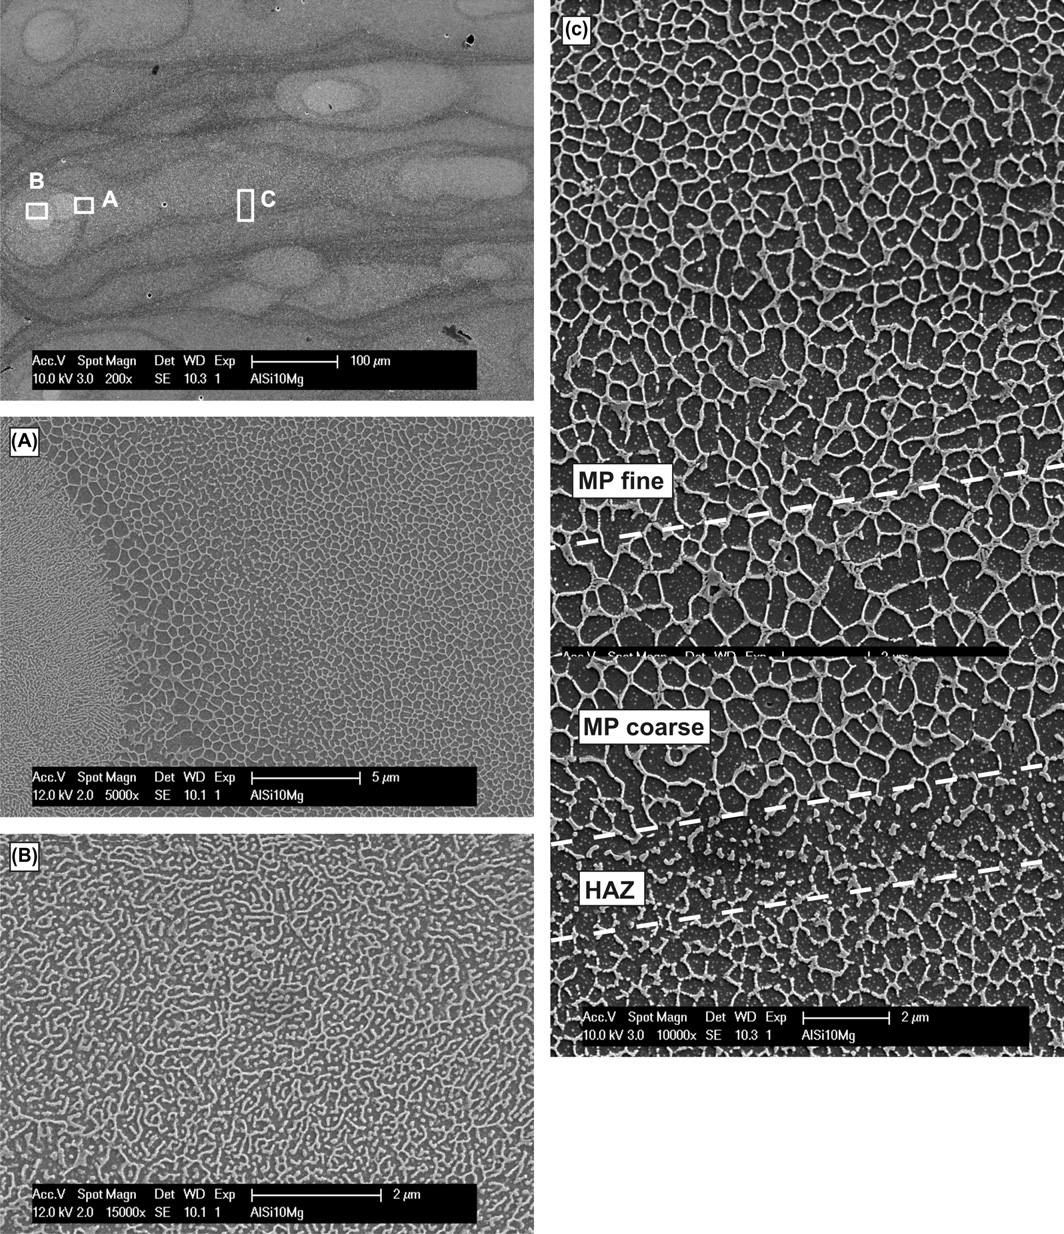
\includegraphics[scale=0.40]{Images/micro_am}
	\decoRule
	\caption[Top view of the microstructure of an Al-Si alloy manufactured by SLM at different scales. Locations of pictures (a), (b) and (c) appear on the top left picture]{Top view of the microstructure of an Al-Si alloy manufactured by SLM at different scales. Locations of pictures (a), (b) and (c) appear on the top left picture (from Thijs et al., 2013 \parencite{Thijs13}).}
	\label{fig:micro_am}
\end{figure}

\begin{figure}[ht]
	\centering
	\includegraphics[scale=0.60]{Images/microTT}
	\decoRule
	\caption[(a) The microstructure of selective laser melted AlSi10Mg after annealing heat
treatment and (b) solution heat treatment followed by artifi cial aging. (c) Both heat
treatments promoted spheroidization phase transformation. ]{(a) The microstructure of selective laser melted AlSi10Mg after annealing heat
treatment and (b) solution heat treatment followed by artifi cial aging. (c) Both heat
treatments promoted spheroidization phase transformation (from Aboulkhair et al., 2017 \parencite{aboulkhair2017}).}
	\label{fig:microTT}
\end{figure}

\section{Fabrication process parameters}
\label{pp}
Let us now investigate the influence of the parameters on the properties of AlSi10Mg parts manufactured with SLM. The analysis of the paired impacts of the laser power P and scan speed $v_s$ provides a first insight. As depicted by figures \ref{fig:Pvs} and \ref{fig:Pvs2}, low P and high $v_s$ lead to an insufficient energy input to melt the powder and re-melt the substrate, which causes the formation of droplets \parencite{Kempen110817} . The opposite leads to good penetration but also to distortions and irregularities.   A trend to use both high P and $v_s$ rose in accordance with these findings. Doing so has the advantage to increase productivity. However, it also has multiple downsides including a decrease of the surface quality due to balling, excessive spatter, and an augmented gas induced porosity \parencite{Mertens170406}. Therefore, a trade-off must be found. \\

A popular approach is to regroup multiple operating parameters into one; the volumetric energy density $E_d$. It is estimated through the following formula: 
$$E_d=\frac{P}{v_s h t} $$
where t is the layer thickness and h is the hatch space.  Maximisation of $\rho_{rel}$ is obtained for $E_d\simeq $ ranging from 40 to 90 $[\frac{J}{mm^3}]$ \parencite{Trevisan2017}. Read et al. obtained a minimal porosity with $E_d \simeq 60$ $[\frac{J}{mm^3}]$ \parencite{Read150417}. However, chosing a right $E_d$ is insufficient and others phenomena, such as melt pools overlapping, should be considered \parencite{Tang170309}. Very few studies were carried out to optimize h and t independently. Their values lie generally in the intervals [50 ; 200] [$\mu m$] and [20 ; 60] [$\mu m$], respectively \parencite{aboulkhair2016,Brandl121509,Kempen110817,Mertens170406}. It was observed that for t = 30 [$\mu m$], an optimal set of parameters values in terms of density is P = 200 [W], $v_s=1400 [\frac{mm}{s}]$ and h = 105 [$\mu m$] \parencite{Kempen110817}. The apparent relative density $\rho_{a,rel}$ was then above 99.5 [\%], considering the theoretical bulk density $\rho_b$ to be equal to 2.68 [$\frac{g}{mm^3}$].\\

\begin{figure}[ht]
\centering
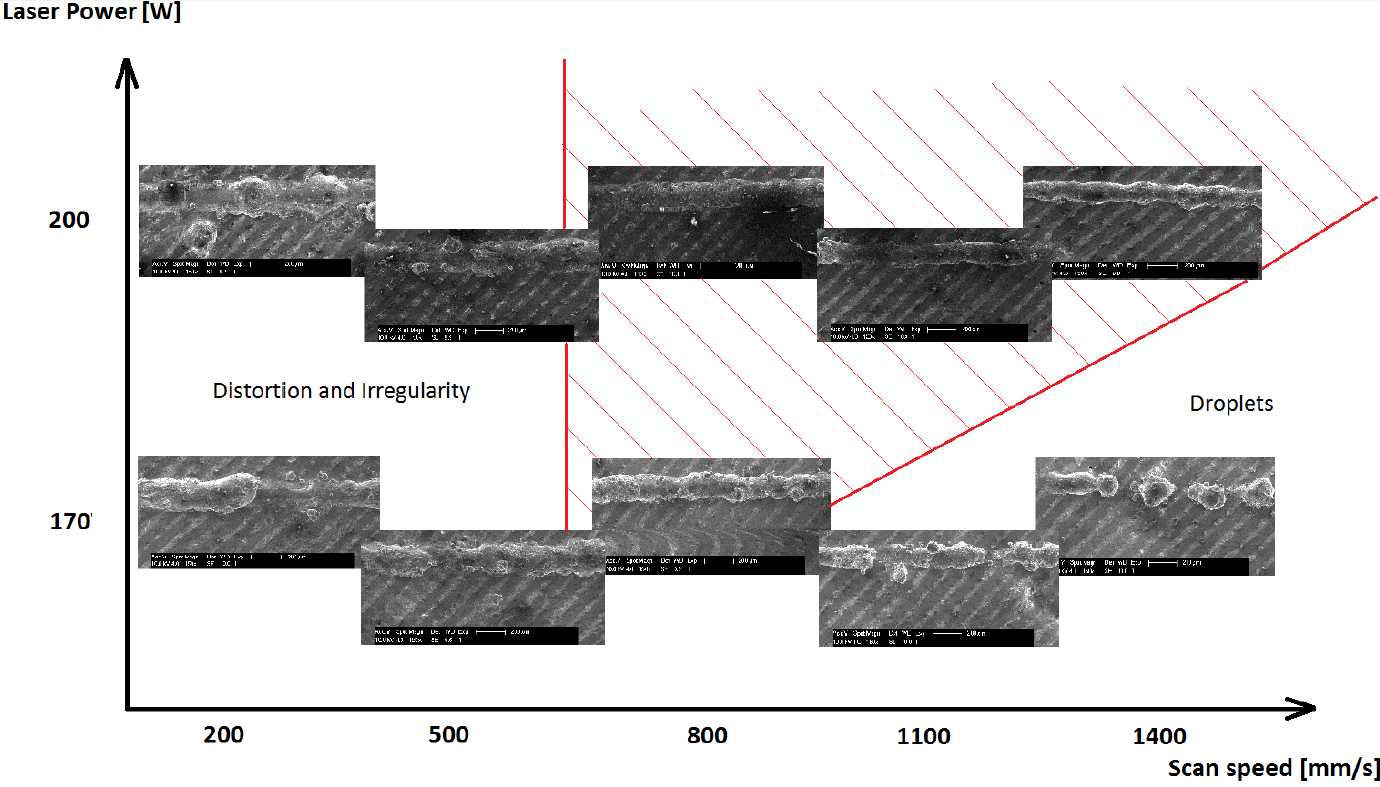
\includegraphics[scale=0.34]{Images/Pvs}
\decoRule
\caption[Process window for SLM of AlSi10Mg, based on the top view of single track scans]{Process window for SLM of AlSi10Mg, based on the top view of single track scans (from Kempen et al., 2011 \parencite{Kempen110817}).}
\label{fig:Pvs}
\end{figure}

\begin{figure}[ht]
\centering
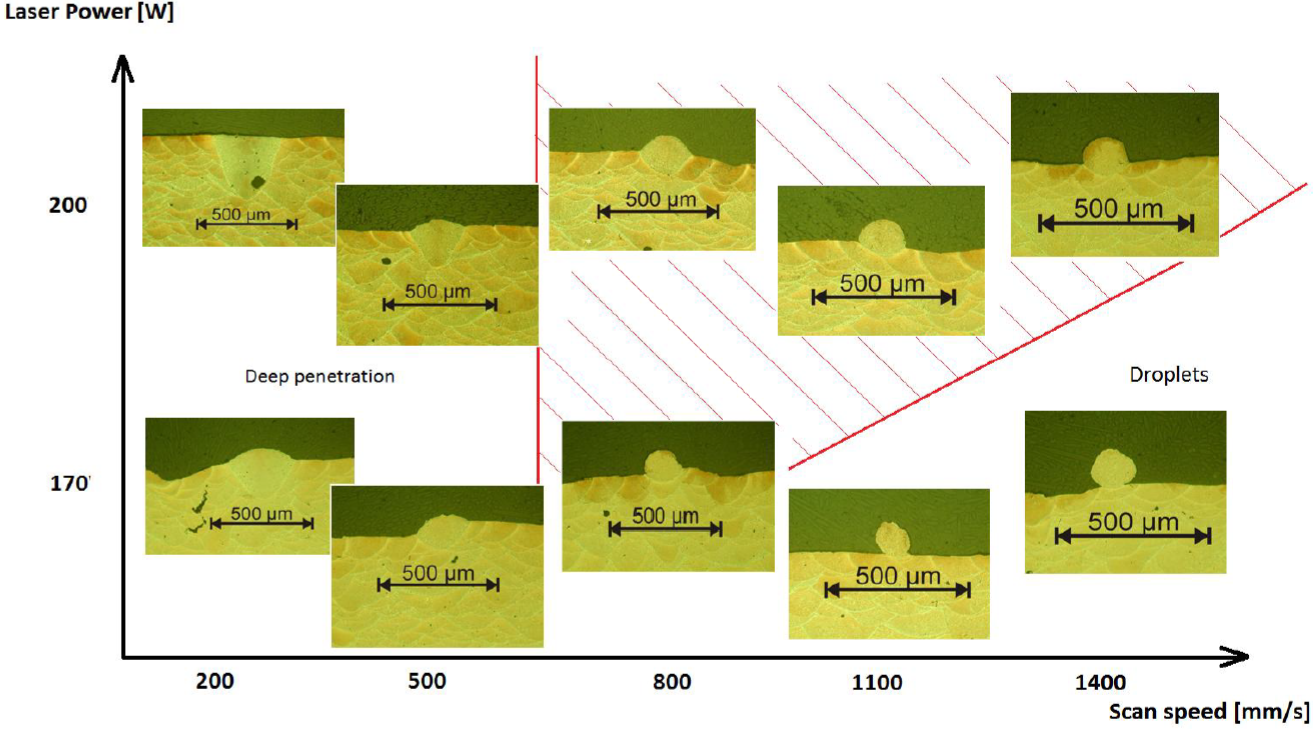
\includegraphics[scale=0.34]{Images/Pvs2}
\decoRule
\caption[Process window for SLM of AlSi10Mg, based on the front view of single track scans]{Process window for SLM of AlSi10Mg, based on the front view of single track scans (from Kempen et al., 2011 \parencite{Kempen110817}).}
\label{fig:Pvs2}
\end{figure}

The other process parameters will be covered for the sake of completeness. Let us first look into the particle-related parameters. The particle size $D_a$ of the powder should be as small as possible to ensure a good flowability and allow for thin layers \parencite{Kempen110817}. Typical values for mean particle size stretch from 15 to 50 [$\mu m$] but are more often at around 30 [$\mu m$] \parencite{Brandl121509,Kempen110817,MOWER2016198,UZAN2017229}. The size distribution is more delicate to outline. On one hand, wider distributions often generate better bed density, parts with higher density and better surface finish. On the other hand, narrower ones usually provide better flowability and parts with better strength and hardness \parencite{Liu1101}. In most cases, a middle ground between the two should be sought. In SLM applications, powder is often successively recycled multiple times. This leads to their progressive contamination with moisture, which causes an increase of hydrogen porosity in the produced parts \parencite{Weingarten151102}. The problem can be overcome by drying the powder or using fresh one. Unfortunately - in the case of aluminium alloys - no findings were made regarding the prediction of a threshold at which one should take action \parencite{aboulkhair2017}.    \\

The choice of scan pattern has great importance. There exist a few different strategies. The common ones use unidirectional, bidirectional or islands patterns (see figure \ref{fig:Strat}). The scan direction(s) should always be rotated between successive layers to favorise isotropy, especially in the unidirectional case since it causes height variations along a layer \parencite{aboulkhair2016}. The islands pattern is based on a decomposition in small domains with short scanning tracks. Two usual strategies can be distinguished among this group: the chessboard and the hexagonal one. A study proved the superiority of an island pattern over a bidirectional one in terms of both ultimate tensile stress $\sigma_u$ and strain at fracture $\epsilon_f$ for a 316L stainless steel-Inconel 718 material \parencite{Zhou15}. It was also shown that it was possible to fabricate pure titanium samples without cracks using an island pattern, and not with a bidirectional one \parencite{Li17}. This is seemingly due to the greater accumulation of internal stresses and to the weaker interlayer bounding in the second case. \\

\begin{figure}[ht]
\centering
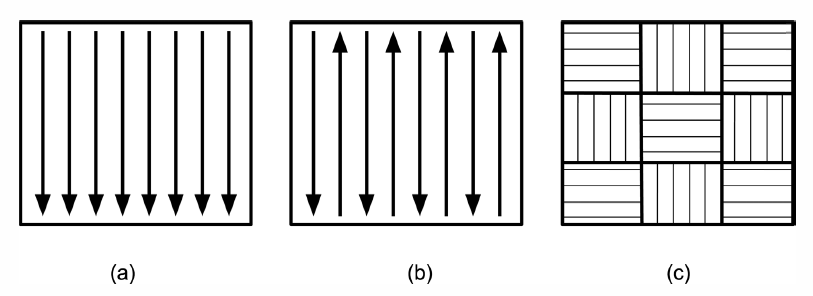
\includegraphics[scale=0.6]{Images/Strat}
\decoRule
\caption[Schematic representation of scanning strategies commonly used in LSM (a) unidirectional long scan track; (b) bi-directional long scan track, and (c) islands]{Schematic representation of scanning strategies commonly used in LSM (a) unidirectional long scan track; (b) bi-directional long scan track, and (c) islands (from Mertens et al., 2017 \parencite{Mertens170406}).}
\label{fig:Strat}
\end{figure}

Furthermore, dual scanning strategies were proven to be effective. For example, a pre-scan with low $E_d$ can flatten the powder bed before it is consolidated, which leads to a reduction of porosity \parencite{Mertens170406}. It was also shown that scanning the contour of the part being built at lower $E_d$ can better the surface roughness for AlSi12Mg \parencite{PRASHANTH170205}. One should note too that the final properties of the fabricated part can strongly depend on the building direction (see figure \ref{fig:Build}) \parencite{DELROISSE201732}. Further properties comparison is provided in section \ref{MMABMP}.\\

\begin{figure}[ht]
\centering
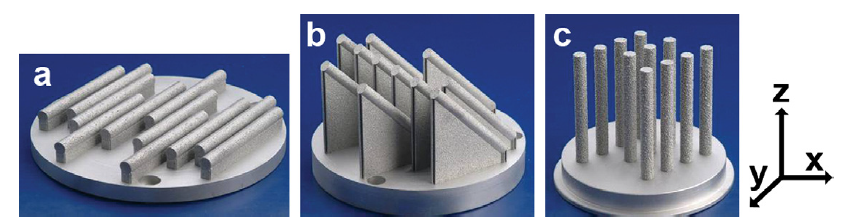
\includegraphics[scale=0.58]{Images/Build}
\decoRule
\caption[Samples (static tensile) built in different directions: (a) $0^\circ$, (b) $45^\circ$, and (c) $90^\circ$]{Samples (static tensile) built in different directions: (a) $0^\circ$, (b) $45^\circ$, and (c) $90^\circ$ (from Brandl et al., 2012  \parencite{Brandl121509}).}
\label{fig:Build}
\end{figure}


Other laser-related parameters - the spot size and the pulse properties - can also influence the process. Only the laser spot size at the 99\% contour $\phi_{99\%}$ is frequently cited in literature. Its value lies between 20 and 200 [$\mu m$] \parencite{Brandl121509,Kempen110817,MOWER2016198}. At this moment, no optimisation study was carried out about this variable. One should expect the optimal value for P, $v_s$, t, and h to depend on the spot size as it has a direct incidence on $E_d$. \\

Finally, the temperature of the powder bed and feeder affect the final properties of the fabricated parts as well. In particular, it was observed that pre-heating the powder at $300^\circ$ C mitigates the differences of fatigue resistance between tensile specimens built in different directions: it is possible that the operation induces a slower cooling rate which helps reducing the distortions and internal stresses \parencite{Brandl121509}.\\

Once the porosity problem is sorted out, other matters can be addressed such as productivity and surface roughness. The latter is problematic as the surface finish obtained with SLM is typically of such poor quality that all cracks initiate near the surface for a sample with relative density $\rho_{rel}>99\%$ \parencite{Brandl121509}. As said before, it is possible to reduce the surface roughness by mean of a dual scan strategy. However, the only options to obtain significantly better surface finish is currently to machine or polish the fabricated parts. This is one of the main weak points of SLM.\\ %Durant les dernières années, les travaux visant à optimiser les conditions de fabrication se sont multipliés. La minimisation de la porosité est au centre de l'attention: elle est en effet liée à la qualité des propriétés mécaniques. De plus au delà d'un seuil, des risques de rupture prématurée peuvent apparaitre (source). (Initiation de sites de propag ... ) On s'intéresse ensuite à optimiser d'autres caractéristiques du matériau et à la productivité de la technique.


\section{As-built mechanical properties}
\label{MMABMP}
In a work of Kempen et al., it was concluded that as-built (AB) additively manufactured AlSi10Mg samples can have mechanical properties (Vickers hardness \textit{HV}, ultimate tensile stress $\sigma_u$ , fracture strain $\epsilon_f$ and impact energy) better or at least comparable to the conventionally casted and high pressure die casted (HPDC) alloy \parencite{KEMPEN2012439}. The tensile specimens built in an horizontal direction (XY) had slightly different characteristics than those built in the vertical direction (Z). The results obtained in the mentioned work are gathered in table \ref{tab:Kemp1}, along with other results and common cast AlSi10Mg properties. The mechanical properties all lie in wide ranges. This illustrates the importance of mastering the process parameters. The best tensile properties measurements found on the web - both in terms of $\sigma_u$ and $\epsilon_f$ - were obtained by \textit{EOS} with $\rho_{rel} \simeq 99.85$  ($\rho_b$ considered to be equal to 2.67 [$\frac{g}{cm^3}$]) \parencite{EOS}. Unfortunately, the manufacturing condtions were omitted in sources \parencite{EOS}, \parencite{KEMPEN2012439} and \parencite{LI2016116}.

 \begin{center}
\begin{table}[ht]
\noindent\makebox[\textwidth]{\begin{tabular}{|c|c|c|c|c|c|}
    \hline
    Process & E [GPa] &$\sigma_y [MPa]$ &$\sigma_u$[MPa]&$\epsilon_f$[\%]&HV [HV] \\
\hline
\hline   
    SLM - XY direction \parencite{KEMPEN2012439}& $68 \pm 3$& - &$391 \pm 6$&$5.55\pm 0.4$&127	\\
    SLM - Z direction \parencite{KEMPEN2012439}& &- &$396 \pm 8$ & $3.47\pm 0.6$&	\\
    SLM  \parencite{ABOULKHAIR2016139}& $77 \pm 5$ & $268 \pm 2$  &$333 \pm 15$ & $1.4 \pm 0.3$ & $125 \pm 1$\\
    SLM - XY direction \parencite{MOWER2016198} & 65.5 & 227 &358&3.9 & - \\
    SLM - Z direction \parencite{MOWER2016198} & 75.4 & 172 & 289 & 2.6 & - \\
    SLM - XY direction \parencite{EOS} & $75 \pm 10$ &$270 \pm 10$ &$460 \pm 20$ &$9 \pm 2$ & $ 119 \pm 5$  \\
    SLM - Z direction \parencite{EOS} & $70 \pm 10$ &$240 \pm 20$ & $460 \pm 20$   &$6 \pm 2 $ &  \\
    SLM \parencite{LI2016116} & - & $322.2 \pm 8.1 $ & $434.3 \pm 10.7 $ & $5.3 \pm 0.2 $ & - \\
    \hline
    Conventional cast and aged \parencite{KEMPEN2012439}& 71 &- &300-317&2.5-3.5&86\\
    As built HPDC \parencite{KEMPEN2012439}& &- &300-350&3-5&95-105\\
    T6 treated HPDC \parencite{KEMPEN2012439}& &- &330-365&&130-133\\
    \hline

\end{tabular}}

\caption[Mechanical properties of SLM built parts and cast + aged parts in literature]{Mechanical properties of SLM built parts and cast + aged parts in literature}
\label{tab:Kemp1}
\end{table}
 \end{center}
 
Furthermore, Wang et al. observed that preheating the manufacturing plate can have great impact on the mechanical properties \parencite{Wang2018}. This is due to the differences in thermal gradients between the substrate and the built samples, which induces residual stresses. Results obtained for a chessboard pattern are shown in table \ref{tab:Wang}. Residual stresses are discussed further in section \ref{EARSSP}.

 \begin{center}
\begin{table}[ht]
\noindent\makebox[\textwidth]{\begin{tabular}{|c|c|c|c|c|}
    \hline
    Plate temperature &$\sigma_y$ [MPa] & $\sigma_u$ [MPa] & $\epsilon_f [\%]$  & $\rho_{rel} [\%]$ \\
\hline
\hline   
    80$^\circ C$&176 $\pm 6$ &385 $\pm 6$ & $3 \pm 1.5$ & 98.69 $\pm 0.19$	\\
    120$^\circ C$ &257 $\pm 9$&381.3 $\pm 3.3$ & $2.83 \pm 0.33$ &  97.39 $\pm 0.38$	\\
    160$^\circ C$ &233 $\pm 4$&363.7 $\pm 11.3$ & $5.33 \pm 0.67$ &  97.01	\\
    \hline

\end{tabular}}
\caption[Mechanical properties for different plate pre heating temperatures.]{Mechanical properties for different plate pre heating temperatures (from Wang et al., 2018) \parencite{Wang2018}.}
\label{tab:Wang}
\end{table}
 \end{center}

SLM AlSi10Mg is sometimes compared to wrought Al6061. It is also an aluminium-based alloy containing magnesium and silicon as major alloying elements. Its properties (after T6 treatment) are similar to its counterpart's as it is shown in table \ref{tab:6061}. It could thus be considered as an alternative for given applications. Fatigue properties of SLM AlSi10Mg where observed to be substantially poorer to the other material's: its lifetime was approximately one order of magnitude less for any applied stress amplitude (see figure \ref{Fat}) \parencite{MOWER2016198}. It was proven that defects control its fatigue life. The defects giving rise to failure often locate near the surfaces of the samples. %Polishing can thus better their fatigue strength (but not systematically). 
\\

 \begin{center}
\begin{table}[ht]
\centering
\begin{tabular}{|c|c|c|c|c|}
    \hline
    E [GPa] &$\sigma_y [MPa]$ &$\sigma_u$[MPa]&$\epsilon_f$[\%]&HV [HV] \\
\hline
\hline   
    68.9 &276  & 310 &12 &107	\\
    \hline

\end{tabular}
\caption[Mechanical properties of T6 treated Al6061 alloy]{Mechanical properties of T6 treated Al6061 alloy (from Aerospace Specification Metals Inc., 2000 \parencite{6061}) }
\label{tab:6061}
\end{table}
 \end{center}
 
\begin{figure}[ht]
\centering
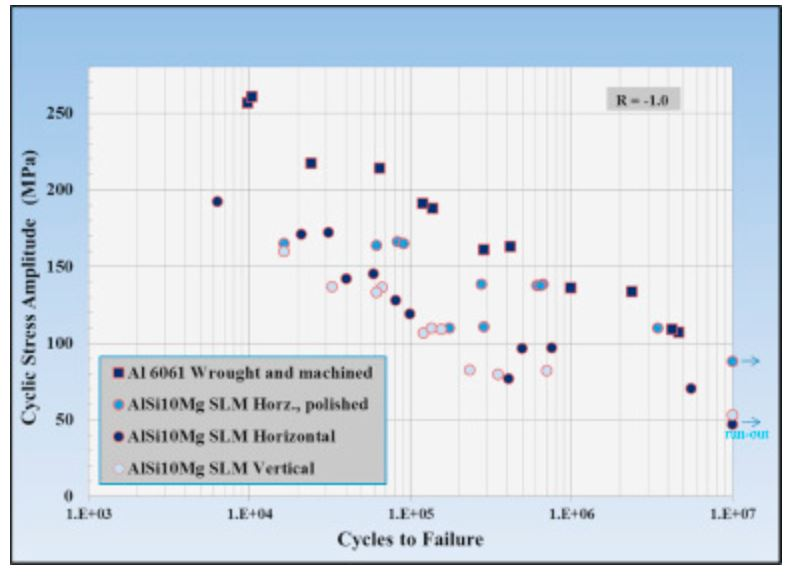
\includegraphics[scale=0.5]{Images/Fat}
\decoRule
\caption[Measured room-temperature stress-life (S–N) of SLM AlSi10Mg, compared to that of conventional Al 6061. Bending fatigue (rotating beam) at a frequency of 25 Hz. ]{Measured room-temperature stress-life (S–N) of SLM AlSi10Mg, compared to that of conventional Al 6061. Bending fatigue (rotating beam) at a frequency of 25 Hz. (from Todd Mower and Michael Long, 2016 \parencite{MOWER2016198}) .}
\label{Fat}
\end{figure} 
 
% \begin{center}
%\begin{table}[ht]
%\noindent\makebox[\textwidth]{\begin{tabular}{|c|c|}
%    \hline
%    Process & Impact energy [J] \\
%\hline
%\hline   
%    SLM - XY direction & $3.94 \pm 0.5$	\\
%    SLM - Z direction & $3.69 \pm 0.48	$\\
%    \hline
%    Conventional cast & 2.5-3.0\\
%    \hline
%
%\end{tabular}}
%\caption[Results of Charpy impact testing]{Results of Charpy impact testing (from Kempen et al., 2012)}
%\label{tab:Kemp2}
%\end{table}
% \end{center}

\section{Residual stresses in SLM parts}
\label{EARSSP}
%\textcolor{red}{Introduire les contraintes internes: pourquoi il y en a? Sont-elles quantifiées dans la littérature? Traction/Comp ? Haut/bas? Techniques de caractérisation? Influence sur les précisions géométriques, sur les propriétés méca (statique \& fatigue)? Comment les éviter en cours de process ou supprimer après? =Intro pour section suivante.}\\

After most manufacturing processes, the fabricated piece can present residual stresses (both in compression and tension). While they are sometimes sought in some specific applications, they are more often an unwanted consequence of the process. Uncontrolled internal stresses can in fact deteriorate dramatically the fatigue behaviour of the piece and cause unacceptable deformation as well as premature failure. They indeed facilitate the initiation of crack growth \cite{Vrancken2016}.\\

Many phenomena can be the cause of residual stresses, but it always comes down to inhomogeneous plastic strains. Several forming processes, such as cold rolling, can induce them by applying a non-uniform load. On a more microscopic scale, different reactions to stress between distinct phases or crystal orientations are also able to create those inhomogeneities.\\

In the case of SLM parts, internal stresses are mostly due to the intense thermal gradients appearing during the scan. After the laser passage, the melt pool cools down and begins to solidify. This solidification brings thermal shrinkage of the molten track, which puts it under tensile condition. The continuous shrinking along the scan track concentrates those tension stresses horizontally, in the direction of the scan vectors. Fabrication of successive layers on top, with their own tensile stresses, gradually relaxes the buried layers to the point that they begin to undergo compressive stresses below a certain depth. Vertical tensile stresses on the side surfaces, induced by those horizontal stresses at each layer, still remain after the complete fabrication. An example of the stress distribution in a 2D section of a piece after manufacturing is available in Fig. \ref{fig:rs_section}. According to the supplier \cite{Inconel}, Inconel718 has a yield strength of approximatively 1 GPa. Although residual stresses do not seem to reach it, their value is definitively high enough to completely modify the mechanical behaviour of the piece. In the case of a tensile test, for example, the zone near the surface would enter plasticity way before applying a stress equal to the yield strength. \\

\begin{figure}[ht]
	\centering
	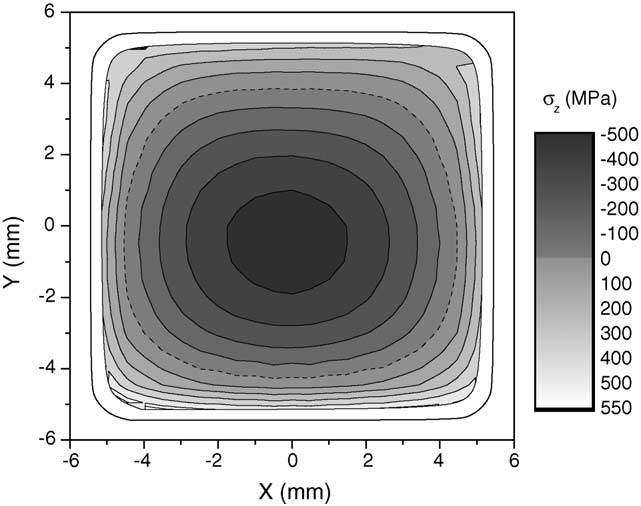
\includegraphics[scale=0.50]{Images/rs_section}
	\decoRule
	\caption[2D plot of vertical internal stresses measured by the contour method at mid-height, in a vertically-built parallelipiped Inconel718 sample. Vertical stresses are null along the dashed line.]{2D plot of vertical internal stresses measured by the contour method at mid-height, in a vertically-built parallelepiped Inconel718 sample. Vertical stresses are null along the dashed line (from Vrancken, 2016 \parencite{Vrancken2016}).}
	\label{fig:rs_section}
\end{figure}

Even though many process parameters influence the amount of residual stresses in the cooled part, reliable quantitative relations are difficult to obtain. On top of that, phenomena specific to the material used - such as the formation of precipitates or the allotropic transformations - restrain us from applying what is known about the process from one material to another. However, the parameter with the most obvious consequences on residual stresses is the powder bed preheating. While it indeed reduces the thermal gradient around the melt pool, and thus reduces internal stresses as well, it is suggested that the lower yield strength at higher temperature is the strongest stress-reducing effect \cite{Vrancken2016}. \\

Another parameter modifying the macroscopic thermal gradient of the part is the presence of building supports, depending on their ability to conduct heat to the platform. Indeed, a part built on a solid support, or directly onto the building platform, has a heat exchange area equal to its section. A honeycomb or another type of hollow support would reduce this area, because the unmelted powder has a much lower heat transfer coefficient\cite{Hodge2014}. Heat generated by the laser would thus escape more slowly out of the part, leading to a higher thermal gradient and, in turn, higher residual stresses \cite{Salmi2017}, as it is shown in Fig. \ref{fig:rs_support}.\\

\begin{figure}[ht]
	\centering
	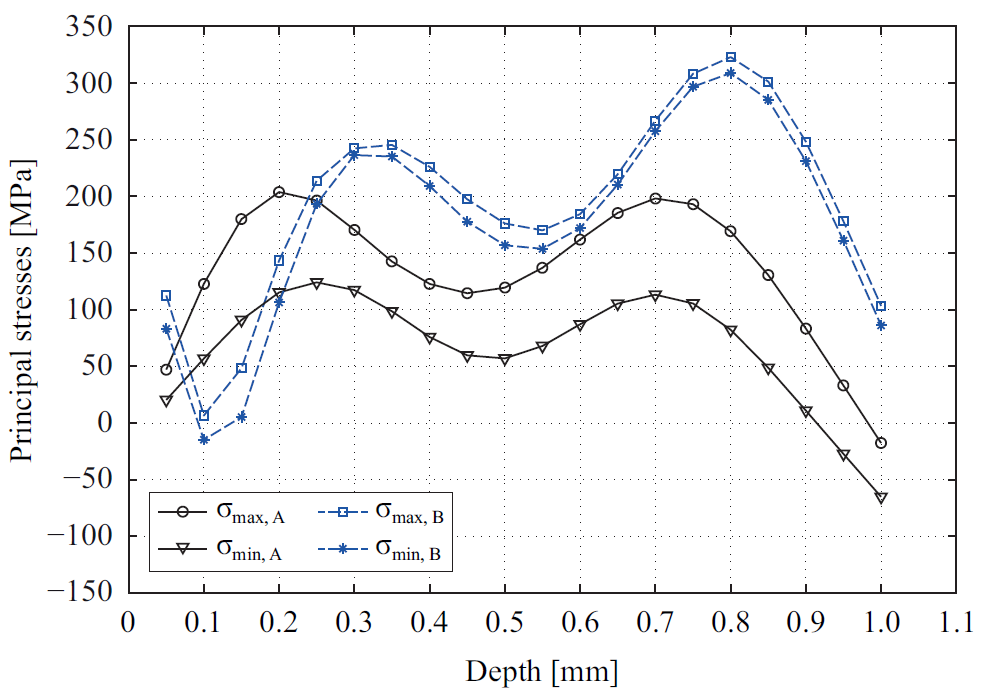
\includegraphics[scale=0.50]{Images/Rs-support}
	\decoRule
	\caption[Principal residual stresses as a function of the depth relative to the surface in a AlSi10Mg part. Sample B is built onto an undefined hollow support, while A is not]{Principal residual stresses as a function of the depth relative to the surface in a AlSi10Mg part. Sample B is built onto an undefined hollow support, while A is not (from Salmi et al., 2017 \parencite{Salmi2017}).}
	\label{fig:rs_support}
\end{figure}

Scanning strategies also play an important in the distribution of residual stesses. Both Kempen et al. (2011) \cite{Kempen110817} and Read et al. (2015) \cite{Read150417} have used an island laser scanning strategy patented by \textit{Concept Laser}, which is supposed to reduce residual stresses in the part \cite{Conceptlaser}. Li et al. (2014) \cite{Li14} relieved stress by applying a dual scan strategy, where a second scan with lower laser energy follows immediately the main fabrication laser passage.\\

Many methods can be used to measure the residuals stresses. They are usually categorised by their destructiveness on the tested part, and their depth of measurement in a reference material; steel. Some of these techniques are presented in Fig. \ref{fig:rs_measure}. The most important non-destructive methods rely on diffraction, which use the lattice deformations at the atomic scale as indicators of the stress the material undergoes. Usual sources of radiation to diffract are X-rays, electrons and neutrons.\\

\begin{figure}[ht]
	\centering
	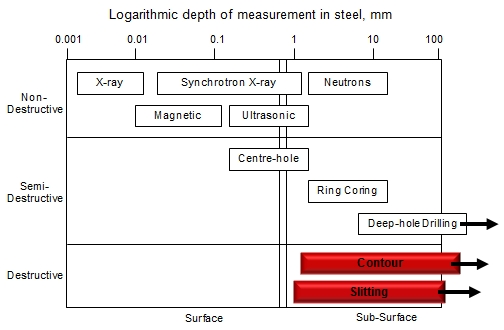
\includegraphics[scale=0.80]{Images/rs_measure}
	\decoRule
	\caption[Non-exhaustive list of residual stresses measurement methods.]{Non-exhaustive list of residual stresses measurement methods (from Hosseinzadeh \parencite{Openuni}).}
	\label{fig:rs_measure}
\end{figure}

A common semi-destructive method is the center-hole drilling. A strain gauge rosette is arranged around a circular area with a diameter of a couple millimetres on a part face. In this area, a shallow cylindrical hole is progressively drilled, increment by increment. The new surfaces formed enable the surrounding material to relax, deforming the hole. The strain gauges records this deformation for each increment. By using the ASTM E837-13a standard \cite{ASTM}, those distortions allow to calculate the residual stresses present in the area before drilling. This method displays practical advantages such as its speed, versatility in term of materials and its ability to do on-site measurements \cite{G2MT}. \\

A fairly recent destructive technique is the contour method (illustrated in figure \ref{fig:rs_section}). It was developed in the early 2000s by Los Alamos National Laboratory \cite{LANL}. The first step, which makes this technique destructive, requires to cut the part in two. The final result of the method is the 2D distribution of residual stresses on the resulting cross-section. This new free surface allows the material to deform and relax some of its stresses. The contour (or shape) of this distorted surface is then measured by using, for example, a Coordinate Measuring Machine (CMM). Then comes the analytical part: a 3D finite-element model of the undeformed cut part is made. A strain with opposite norm to the one measured with the CMM is then applied to the model as a boundary condition, as if we forced the deformed surface back flat. Processing the finite-element results finally gives the stress distribution of the cross section. A visual representation of this calculation is shown in Fig.\ref{fig:contour_meth}\\

\begin{figure}[ht]
	\centering
	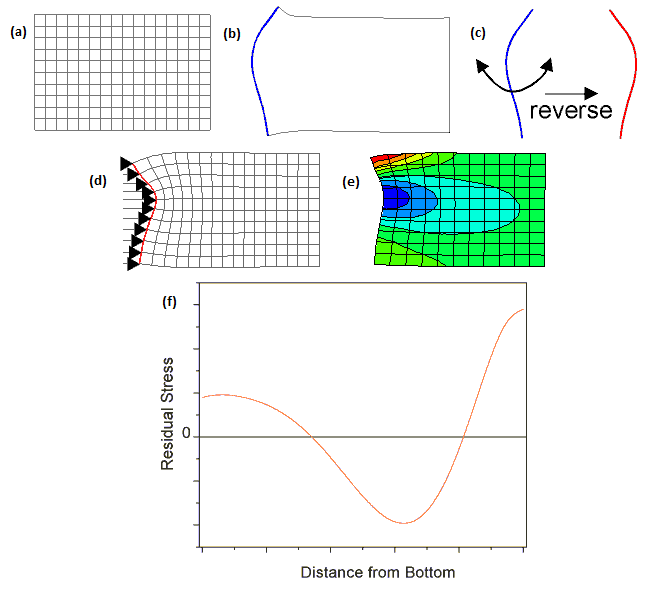
\includegraphics[scale=0.60]{Images/contour_meth}
	\decoRule
	\caption[Thought process of the contour method analytical step]{Thought process of the contour method analytical step: (a)finite-element model of the undeformed part, (b) measured contour of the real part, (c) inversion of strain, (d) application of the strain to the model, (e)resulting stresses in the model, (f) residual stresses normal to the cross section before cutting \parencite{LANL}.}
	\label{fig:contour_meth}
\end{figure}

\section{Post treatments}
\label{SOTAPT}
%\textcolor{red}{Post-traitements habituels en SLM à expliquer: Shot peening, HIP,... dont traitements thermiques, sur lesquels on se focalise. Expliquer + Propriétés mécas après les traitements}
%
%\textcolor{red}{Source que tu peux utiliser:}
%
%\textcolor{red}{Trevisan et al, ‘On the Selective Laser Melting (SLM) of the AlSi10Mg Alloy: Process, Microstructure, and Mechanical Properties’ (AlSi10Mg de manière générale)}
%
%Effet sur microstructure et dureté:
%http://sci-hub.tw/https://link.springer.com/article/10.1007/s11661-015-2980-7
%
%\textcolor{red}{Anne Mertens: 250 deg/2h
%https://orbi.uliege.be/bitstream/2268/185421/1/2015-SFFS-Mertens.pdf}
%
%\textcolor{red}{Traitement T6 \parencite{ABOULKHAIR2016139}}
%
%\textcolor{red}{http://sci-hub.tw/https://www.sciencedirect.com/science/article/pii/S0921509316304890}\\
%
%Impact sur fatigue:
%https://www.sciencedirect.com/science/article/pii/S0264127516306426
%
%Plein de données de littérature
%http://sci-hub.tw/https://www.sciencedirect.com/science/article/pii/S0142112316301463 \\

Unfortunately, although residual stresses can be attenuated as it was discussed above, their presence after the fabrication seems unavoidable. However, cast alloys have known the same problems for their whole history. Various treatments have thus been developed over the years to try to reduce and modify these stresses after the initial manufacturing process. An important part of the literature on SLM alloys has simply studied the effects of those classical heat treatments on AM alloys \cite{Mertens170406}.\\

If the aim is to remove residual stresses, the go-to treatment for aluminium alloys is an annealing at 300$^\circ$C during 2 hours. Data on the heating and cooling speeds are scarce in the literature. Its qualitative effect on the mechanical properties of AM parts is pretty well known and consistent in the literature, at least compared to other treatments. A summary of its effects is presented in Fig. \ref{fig:mech_annealing} \cite{PRASHANTH14}, for different temperatures. The annealing temperature can be varied to obtain a wide spectrum of properties, in order to be better suited for new applications. This treatment reduces strength, both ultimate and yield, while increasing ductility, and this effect is reinforced with rising temperature (at least below 500$^\circ$C). \\

\begin{figure}[ht]
	\centering
	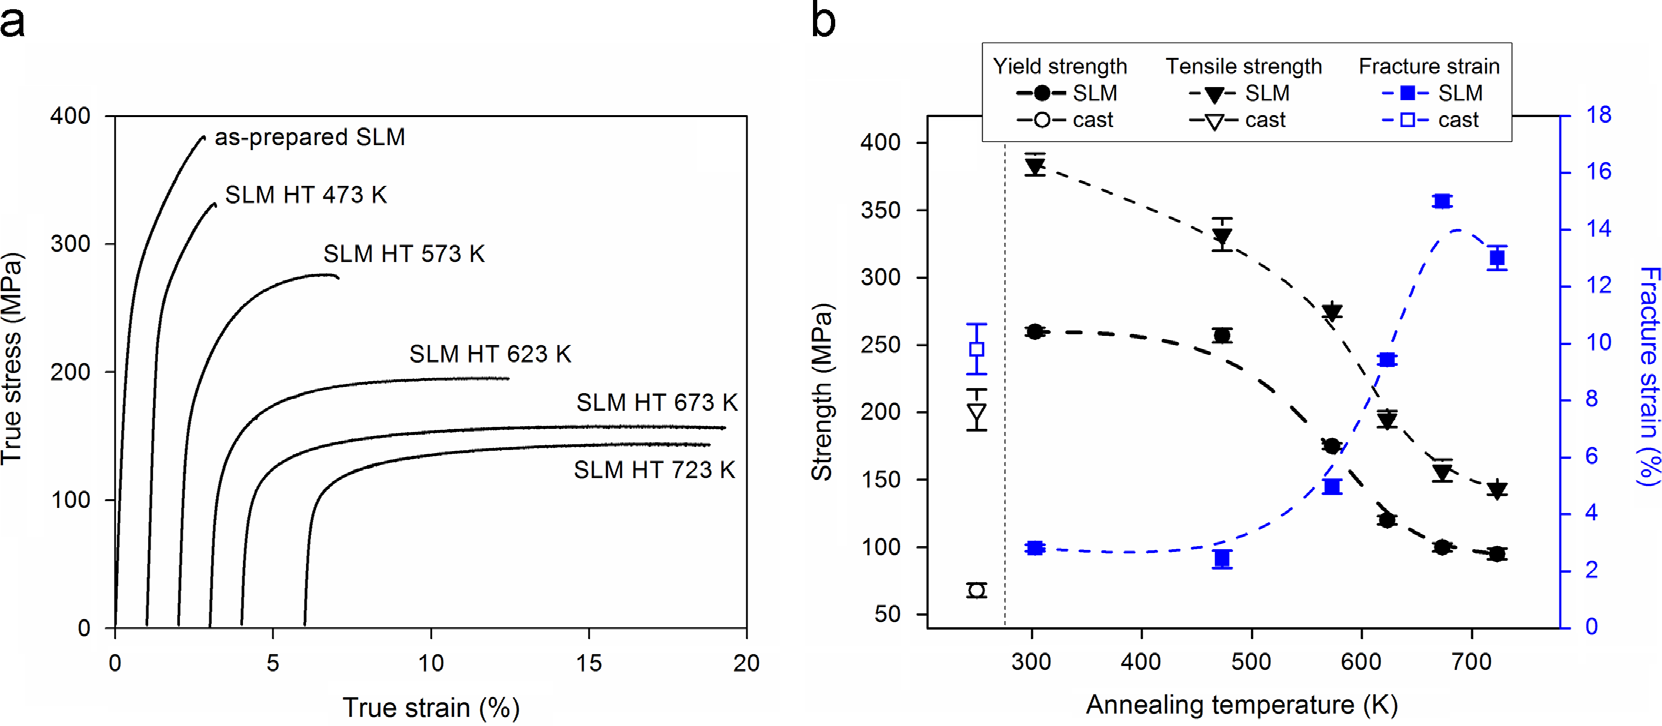
\includegraphics[scale=0.30]{Images/mech_annealing}
	\decoRule
	\caption[(a) True strain-stress curves for an AB AlSi12 sample and several heat-treated ones at different temperatures and (b) corresponding mechanical properties]{(a) True strain-stress curves for an AB AlSi12 sample and several heat-treated ones at different temperatures and (b) corresponding mechanical properties (from Prashanth et al., 2014 \parencite{PRASHANTH14}).}
	\label{fig:mech_annealing}
\end{figure}

The annealing, as well as other heat treatments, alter the mechanical properties through 2 different processes. First, it relieves residual stresses. Indeed, yield strength of materials is temperature dependant: in metals, it decreases with it. During heating, residual stresses at some points in the material surpass the declining yield strength. Those points thus deform plastically, lowering the stress they undergo. In the end, the maximum stress remaining in the material is equal to the yield strength at the highest temperature reached. The resulting residual stresses require specific techniques to be assessed as we saw in section \ref{EARSSP}.\\

Annealing at a sufficient temperature can also modify the microstructure of the alloy. This can be directly observed by optical or electronic microscopy. Mertens et al. (2015)\cite{Mertens15} obtained a very good trade-off, when applying an annealing at 250$^\circ$C for 2 hours with a loss of only 10\% of yield strength and barely 2\% of UTS, the elongation at break increased by 80\%. \\

A very common heat treatment of aluminium alloys is designated by the T6 acronym. It consists of a solution heat treatment around 520$^\circ$C for a variable duration, followed by a water quenching to room temperature and an artificial ageing for several hours between 150 and 190$^\circ$C. When applied to conventionally processed aluminium-based materials, this treatment usually has a hardening effect. The principle is the following \cite{T6}: first step increases solubility of alloying elements in the Al-phase. Water quenching prevents these elements from exiting the phase during cooling, creating a roughly homogeneous super-saturated solution. The artificial ageing finally allows them to slowly diffuse out of the aluminium lattice, forming homogeneously distributed very fine precipitates, hardening the alloy. However, Aboulkhair et al. (2015) \cite{aboulkhair2015}, as well as others, have shown that AM alloys react very differently to this treatment: softening was observed rather than hardening. They suggested that it is due to the dissimilar starting microstructures. T6 heat treatment forms precipitates, but coarsen the AM alloy microstructure at the same time. The strengthening due to the microstructure refinement outweighs in fact the one due to precipitation. This softening means however a higher ductility, and thus a better fatigue strength. A summary of the consequences of T6 heat treatment can be found in Table \ref{tab:ABvsT6}. \\

\begin{table}[ht]
		\centering
			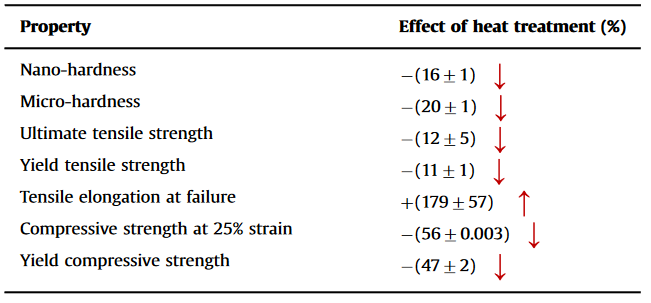
\includegraphics[scale=0.70]{Images/ABvsT6}
			\decoRule
		\caption[Changes in percentage of the main mechanical properties of SLM AlSi10Mg after T6 treatment, , compared to their as-built state]{Changes in percentage of the main mechanical properties of SLM AlSi10Mg after T6 treatment, compared to their as-built state (from Aboulkhair et al., 2016 \parencite{ABOULKHAIR2016139}).}
		\label{tab:ABvsT6}
\end{table}

The time and temperature parameters during the solutionizing and the ageing seem to remain determinant in the prediction of the final properties of the treated part. Indeed, according to Mertens et al. (2015)\cite{Mertens15}, a T6-like treatment can result in an increase of ductility - of course - but also of yield strength. To be complete, they obtained a decrease of hardness of 28\%, a decrease of ultimate tensile strength by 13\%, but an increase of elongation at break of 220\% and of yield strength of 30\%. The distinct process parameters could explain the differences: 510$^\circ$ C during 6 hours followed by 4 hours at 170$^\circ$ C for Mertens et al. (2015)\cite{Mertens15}, compared to 1 hour at 520$^\circ$ C and then 6 hours at 160$^\circ$ C. Differences in manufacturing parameters, such as layer thickness and substrate heating, can as well be at cause.\\

\textcolor{red}{J'en veux PLUS}Hot isostatic pressing (HIP) post-treatment is commercially used for cast aluminium and some have tried to transpose it to SLM AlSi10Mg. Sample is put in a furnace at high pressure ($\simeq 100$ [MPa]) and high temperature (above 500$^\circ C$). These conditions lead to the emergence of plastic flow which heal the internal porosity. This can enhance the mechanical properties of the alloy and reduce the properties scatter \parencite{HIP}. Mower et al. (2016) \cite{MOWER2016198} applied HIP at 900$^\circ$C and 102 [MPa] to a Ti6Al4V AM alloy and obtained a large increase of fracture strain and enhanced fatigue strength. Tradowsky et al. (2016) \cite{Tradowsky16} reported the same fracture strain increase for the AlSi10Mg alloy. \\

Non-thermal processes affecting the residual stresses also exist. As we saw in the previous section, tensile stresses near the surface are the most problematic. A purely mechanical treatment able to cancel these is shot-peening. High velocity projectiles, usually metallic or ceramic beads, are used to hit a surface. The impacts deform plastically the top of the part, which tries to stretch in the horizontal direction. This is prevented by the material below, which remains undeformed. The surface layer thus finds itself in a compressive state \cite{Vrancken2016}. If tensile stresses where present near the surface, they get cancelled by the important compressive stresses included in the material. While injecting compression near the surface can already be beneficial, by hindering crack initiation for example, Salmi et al. (2017) \cite{Salmi2017} also obtained a certain degree of homogenization of the stresses all along the examined depth. \\

Lastly, another well-known drawback of AM parts is their mediocre surface finish compared to cast parts. This roughness, as well as the presence of open porosities, is an important cause of the relatively poor fatigue strength because they constitute privileged points of fracture initiation. However, polishing and machining have shown themselves not very efficient at enhancing fatigue behaviour of AM samples. Mower et al. (2016)\cite{MOWER2016198} had mixed results, where Ti6Al4V parts were improved by machining, while AlSi10Mg ones kept poor fatigue properties after mechanical electrochemical polishing. Aboulkhair et al. (2016) \cite{ABOULKHAIR2016bis} obtained lukewarm results as well, with only some improvement at lower stress levels, whereas heat treatments had a much more significant influence. Both concluded that this lack of enhancement was probably due to the numerous defects near the surface, as well as in the bulk, that were impossible to remove through polishing. \\

Although machining the surface does indeed reduce its roughness, it can also expose buried porosities at the same time which creates sites of choice for fatigue cracking. On top of it, polishing and machining may not always prove themselves easy, fast or cheap to apply to complex-shaped AM parts. They most probably also impact the residual stresses. Machining was observed to have a tremendous influence for wrought aluminium \parencite{Denkena2007}. Cutting speed, feed per tooth and cooling were observed to have notable effects but not as critical as the corner radius's (see figure \ref{fig:Mach}). High compression stresses were induced, going up to nearly 300 [MPa].\\

\begin{figure}[ht]
	\centering
	\noindent\makebox[\textwidth]{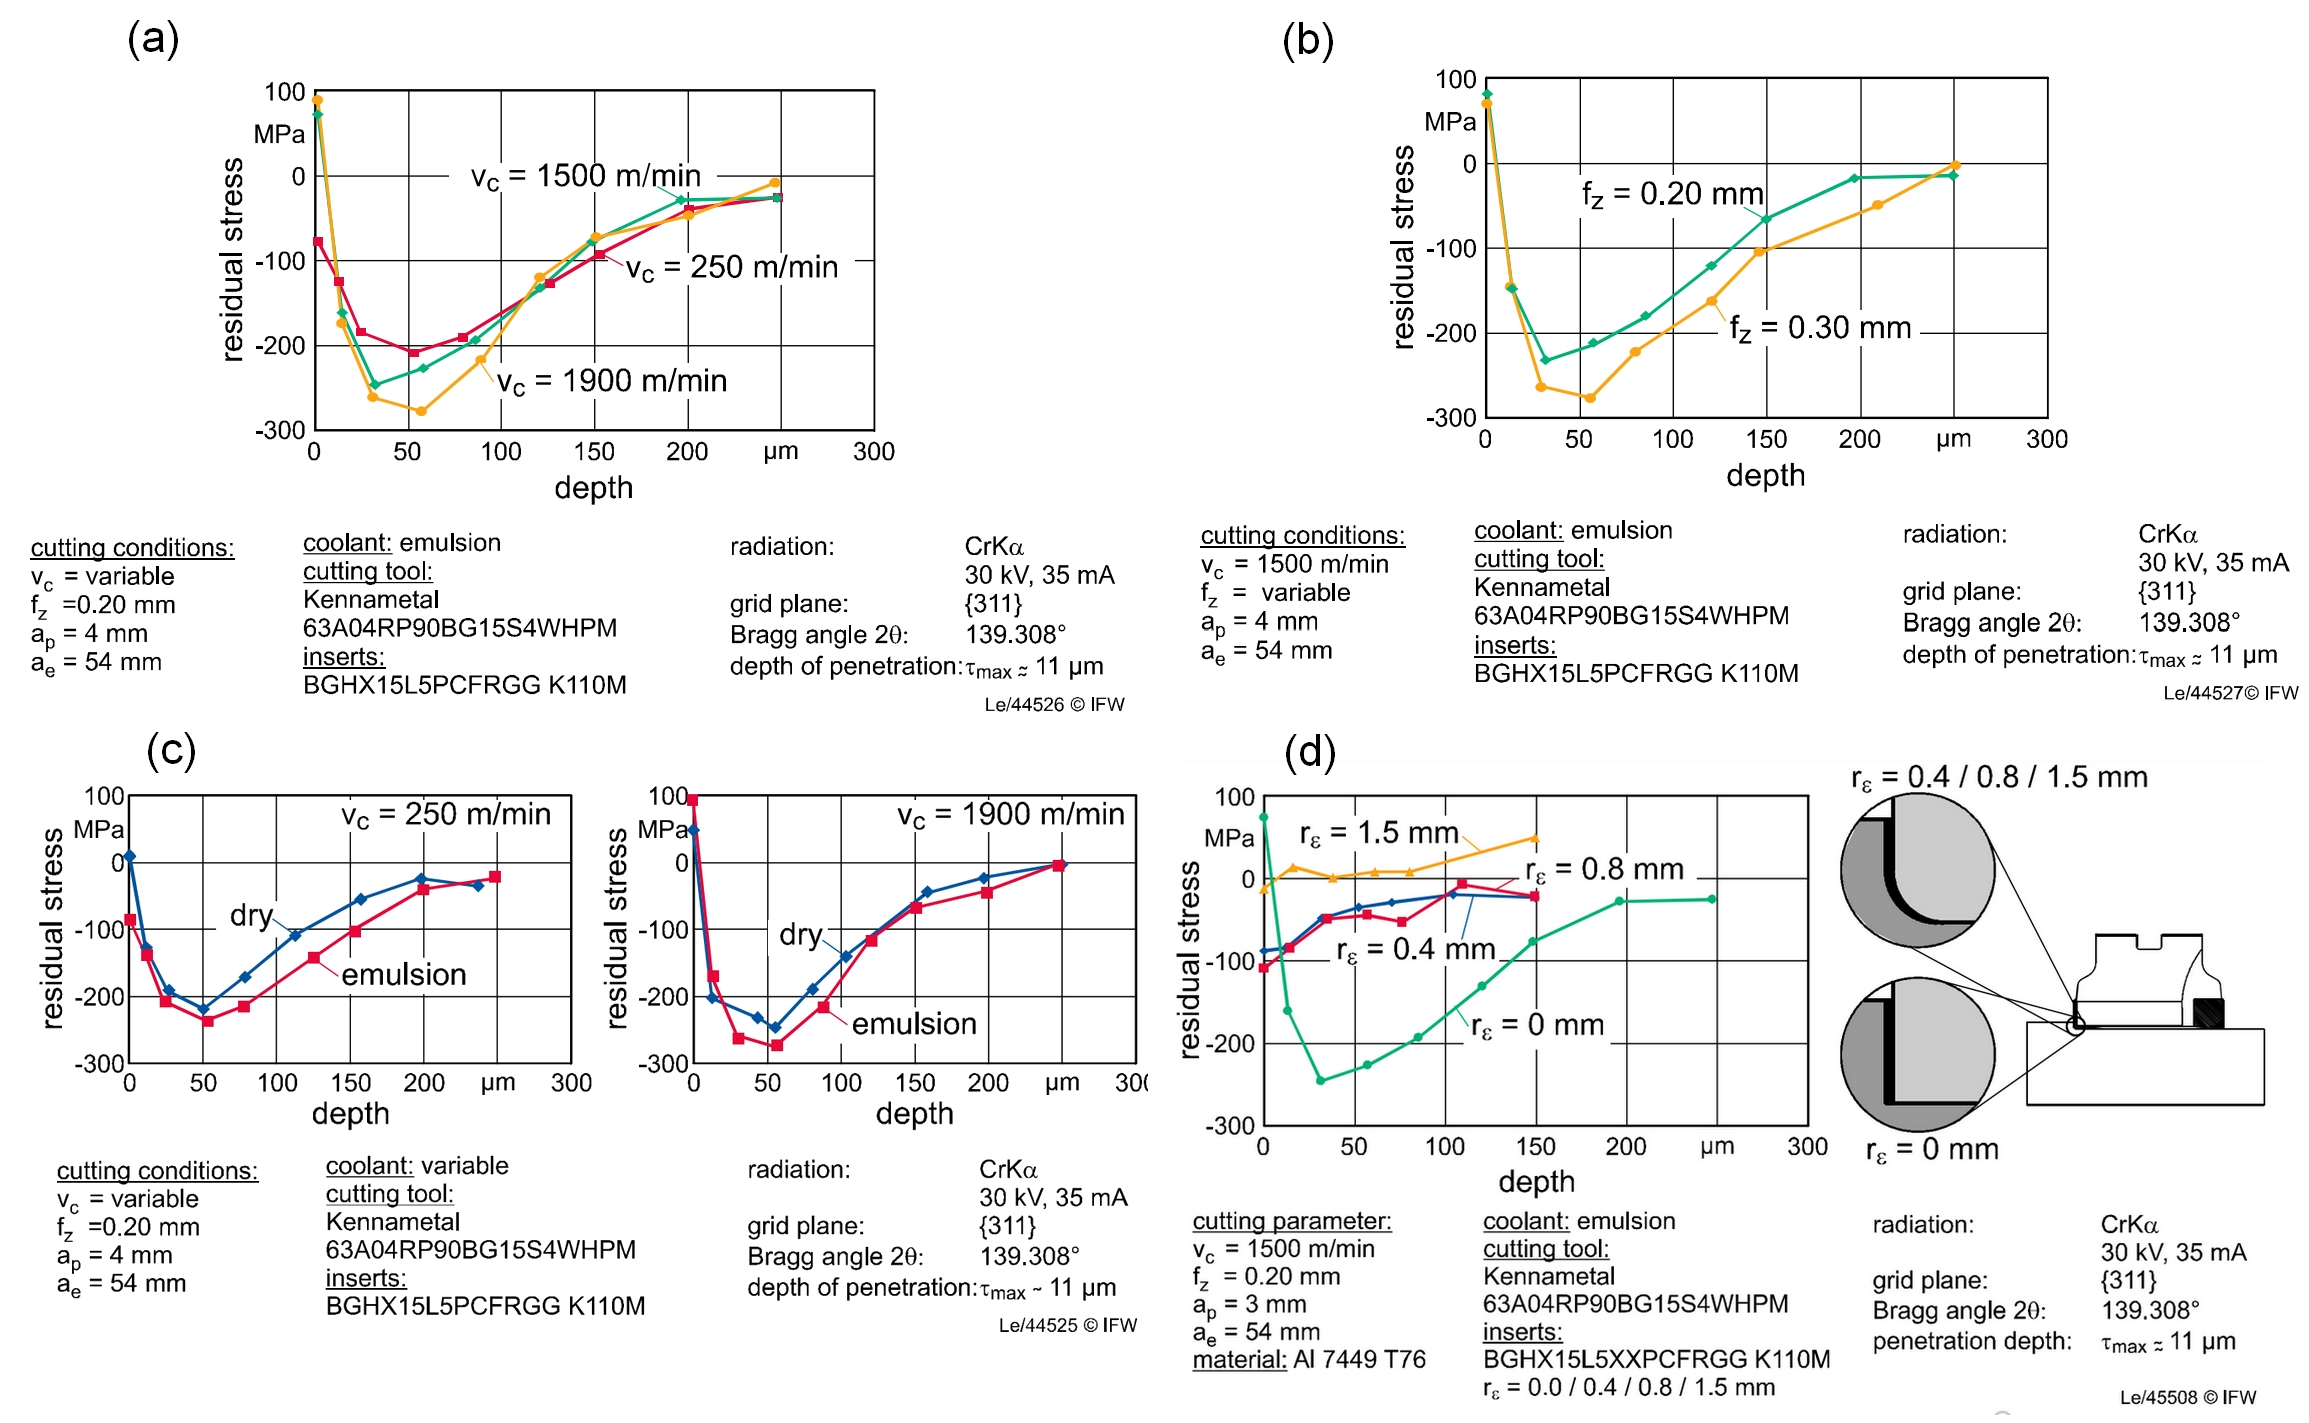
\includegraphics[scale=0.28]{Images/Mach}}
	\decoRule
	\caption[Influence of the cutting parameters on the residual stresses of machined wrought aluminium: (a) cutting speed (b) feed per tooth (c) cooling (d) corner radius.]{Influence of the cutting parameters on the residual stresses of machined wrought aluminium: (a) cutting speed (b) feed per tooth (c) cooling (d) corner radius (from Denkena et al., 2007 \parencite{Denkena2007}).}
	\label{fig:Mach}
\end{figure}

%%ARTICLES SUR LES EFFETS DE L'USINAGE SUR LES CONTRAINTES RESIDUELLES POUR L'ALU :http://www.transport-research.info/sites/default/files/project/documents/20121115_114656_50648_04_IDE_2008_-_Hannover.pdf\\
%
%%http://www.transport-research.info/sites/default/files/project/documents/20121115_114306_73510_CIRP_HSM_2007.pdf\\
%
%%As we saw, 
%
%%Recherches biblio....
%%\section{Comment référencer?}
%%The \code{biblatex} package is used to format the bibliography and inserts references such as this one \parencite{Reference1}. The options used in the \file{main.tex} file mean that the in-text citations of references are formatted with the author(s) listed with the date of the publication. Multiple references are separated by semicolons (e.g. \parencite{Reference2, Reference1}) and references with more than three authors only show the first author with \emph{et al.} indicating there are more authors (e.g. \parencite{Reference3}). This is done automatically for you. %To see how you use references, have a look at the \file{Chapter1.tex} source file. Many reference managers allow you to simply drag the reference into the document as you type.
%%
%%Scientific references should come \emph{before} the punctuation mark if there is one (such as a comma or period). The same goes for footnotes\footnote{Such as this footnote, here down at the bottom of the page.}. You can change this but the most important thing is to keep the convention consistent throughout the thesis. Footnotes themselves should be full, descriptive sentences (beginning with a capital letter and ending with a full stop). The APA6 states: \enquote{Footnote numbers should be superscripted, [...], following any punctuation mark except a dash.} The Chicago manual of style states: \enquote{A note number should be placed at the end of a sentence or clause. The number follows any punctuation mark except the dash, which it precedes. It follows a closing parenthesis.}
%%
%%The bibliography is typeset with references listed in alphabetical order by the first author's last name. This is similar to the APA referencing style. To see how \LaTeX{} typesets the bibliography, have a look at the very end of this document (or just click on the reference number links in in-text citations).